% !TeX root = ..\..\rapport_13_2.tex
\newpage
\appendix
\appendixpage
\addappheadtotoc
\section{Sekvensdiagram: CreateProjectActivity()}\label{apdx:seq_create_project_activity}
\begin{figure}[H]
    \centering
    \caption{Sekvensdiagram: Opret projektaktivitet}\label{fig:sequenceCreateProjectActivity}
    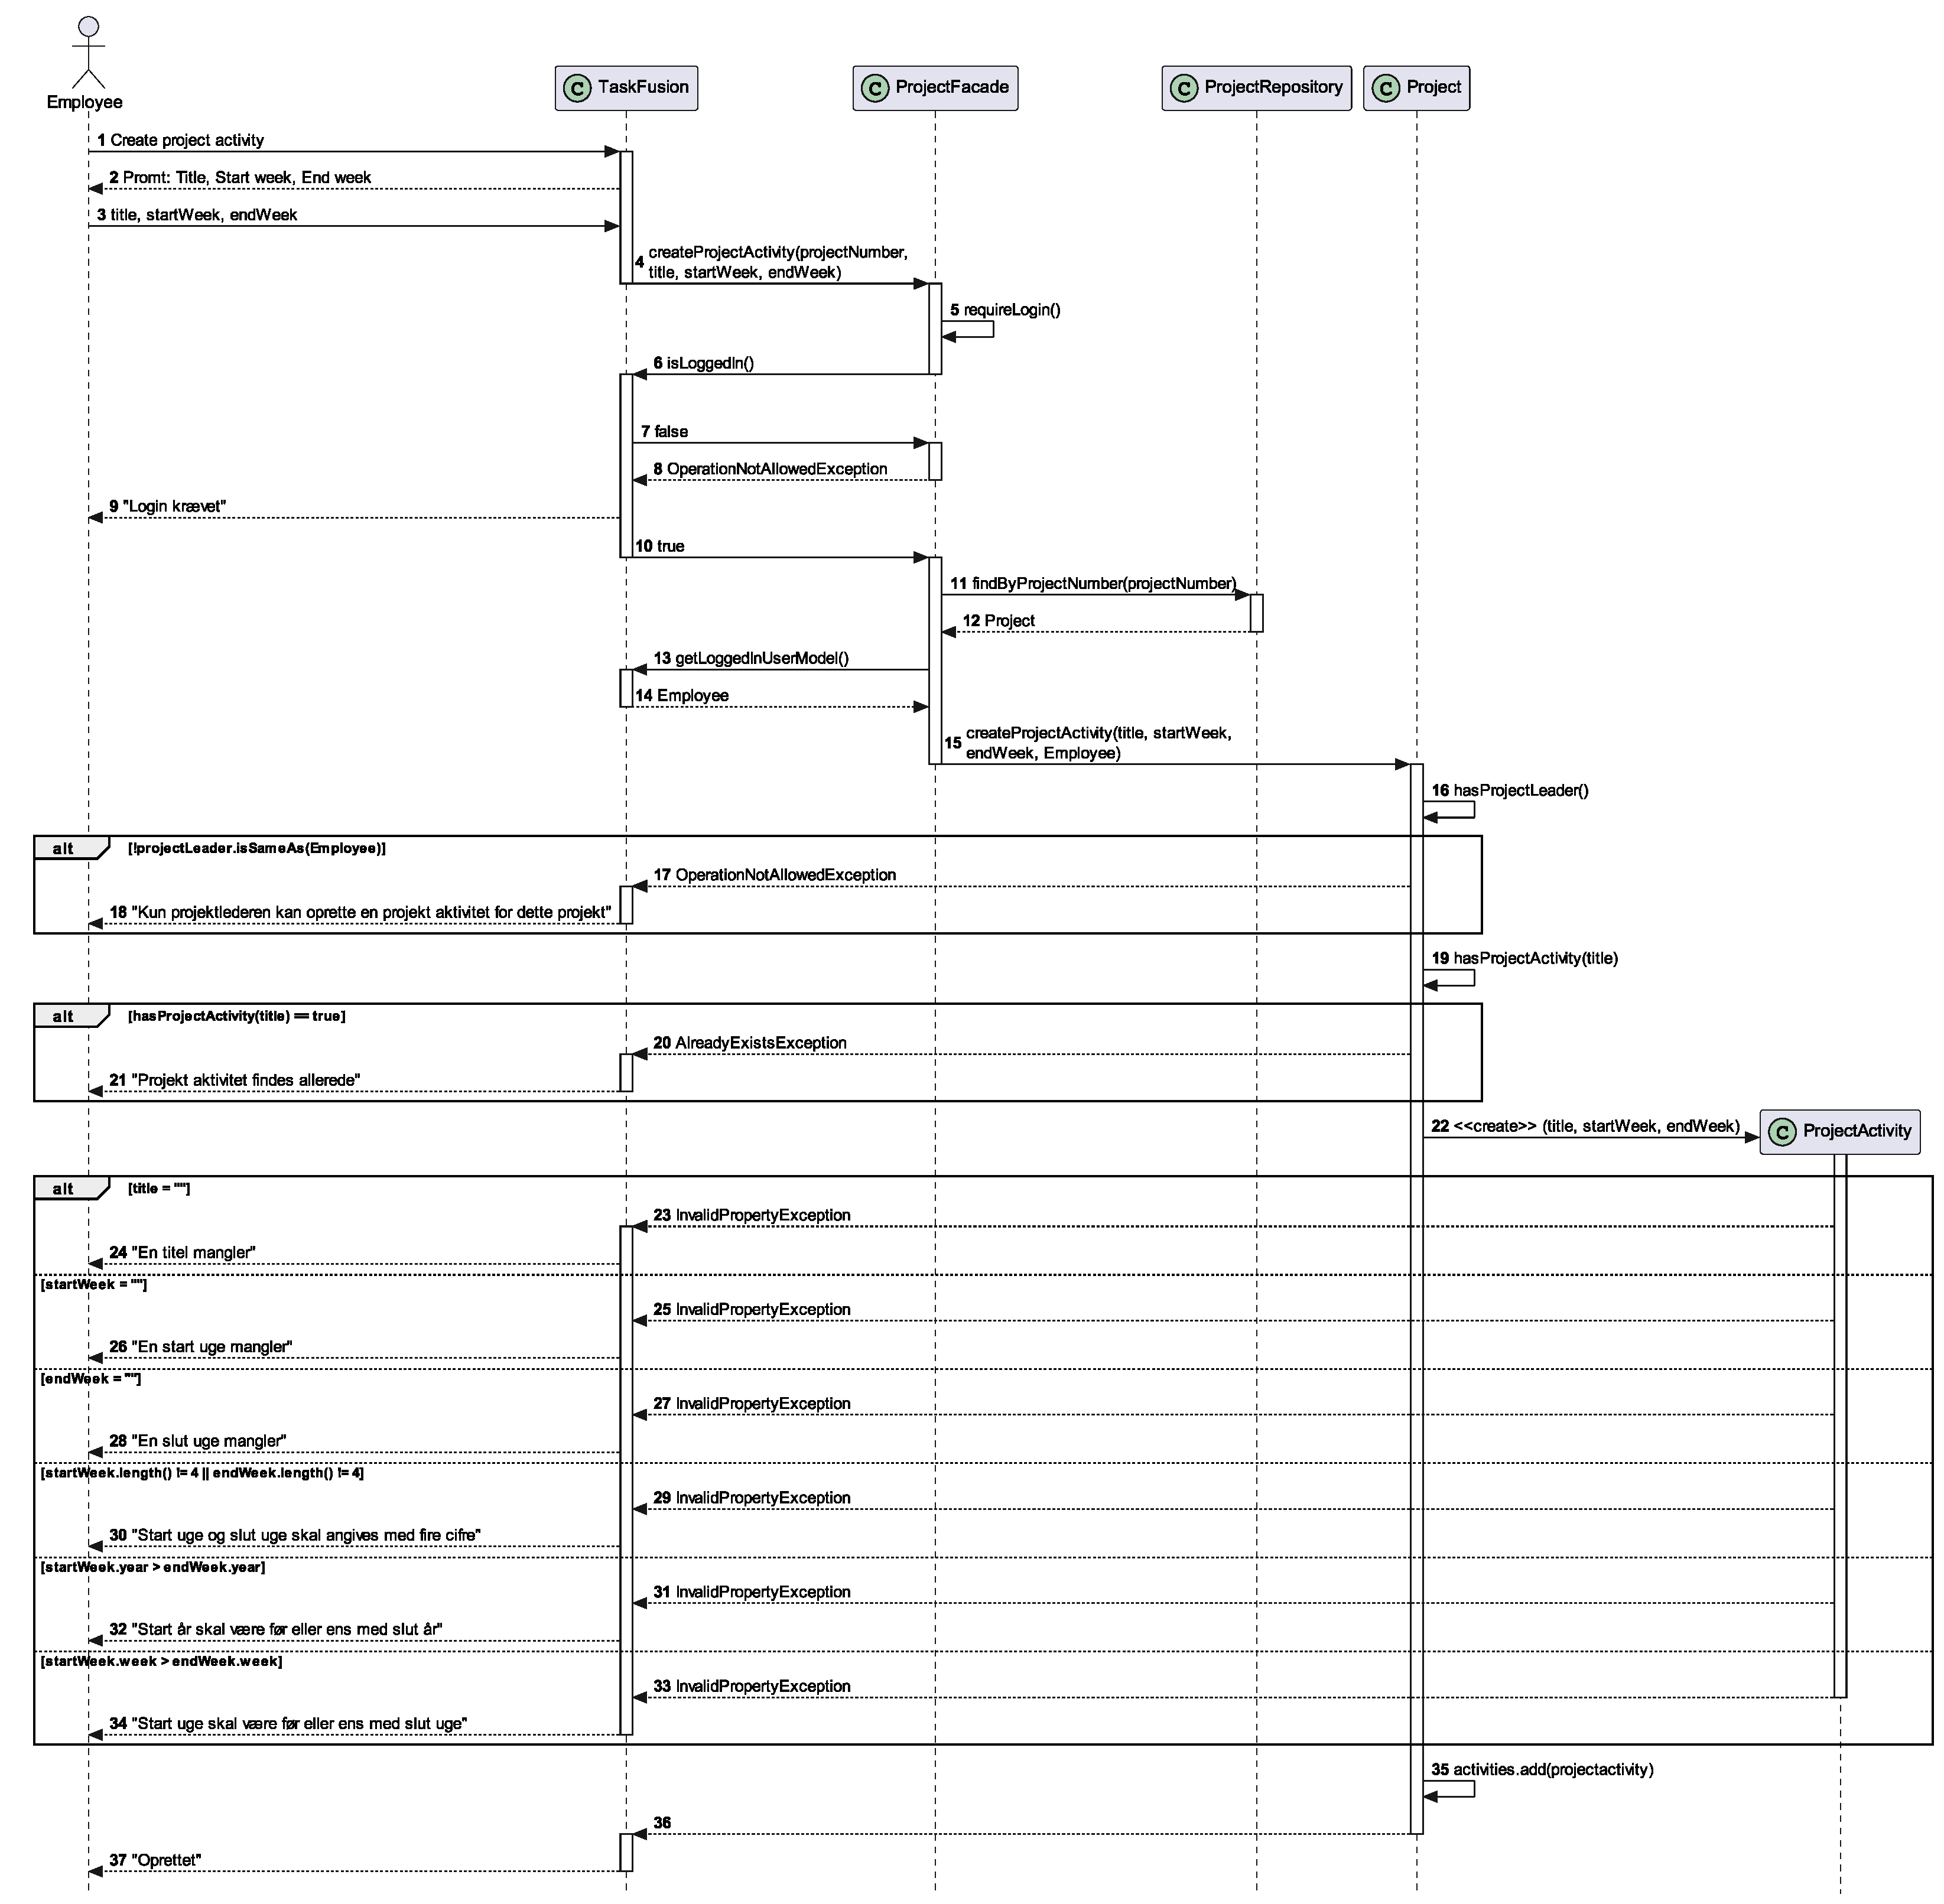
\includegraphics[width=.8\textwidth]{RequirementsAndDesign/SequenceDiagrams/seqCreateProjectActivity.eps}
\end{figure}
\begin{landscape}
    \section{Klassediagram over program laget}\label{apdx:classDiagram_full}
    \begin{figure}[H]
        \centering
        \caption{Klassediagram over program laget}
        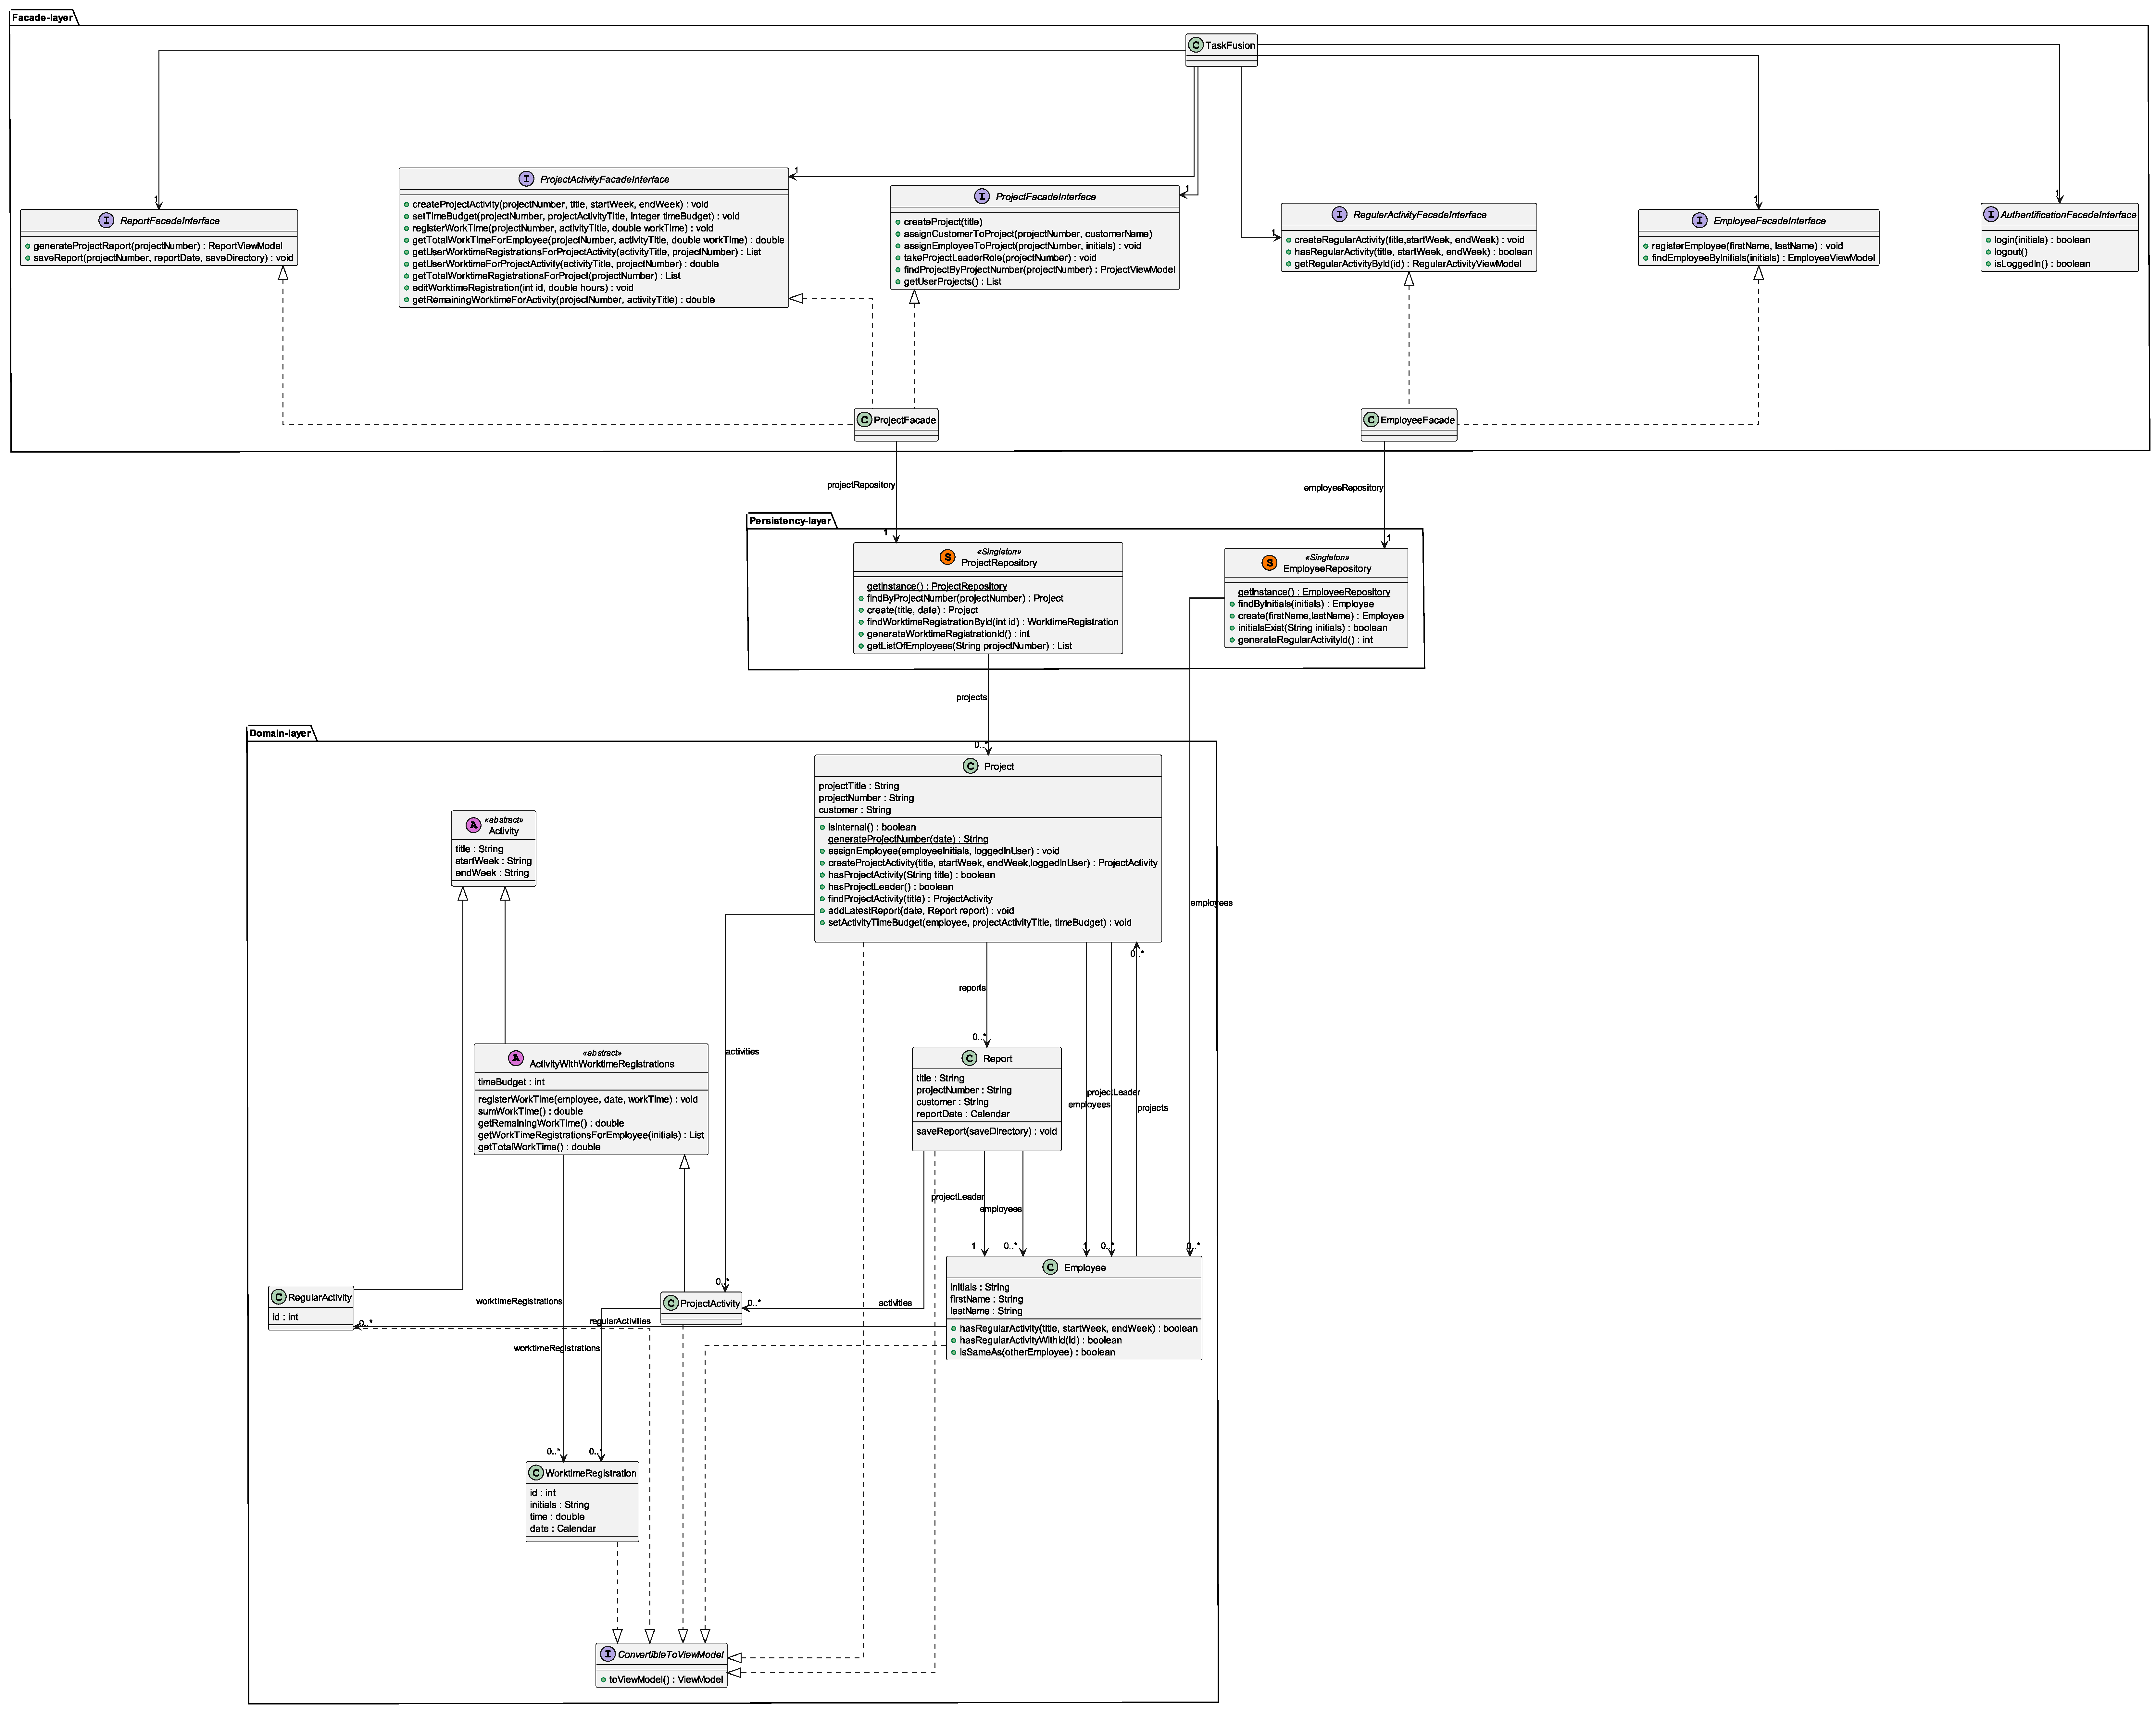
\includegraphics[width = \textheight]{ImplementationAndTest/Diagrams/ClassDiagrams/ClassDiagram_full.eps}
        \label{fig:classDiagram_full}
    \end{figure}
    \section{Klassediagram over præsentations-laget}\label{apdx:classDiagram_presentation}
    \begin{figure}[H]
        \centering
        \caption{Flowdiagram over CLI brugergrænsefladen}
        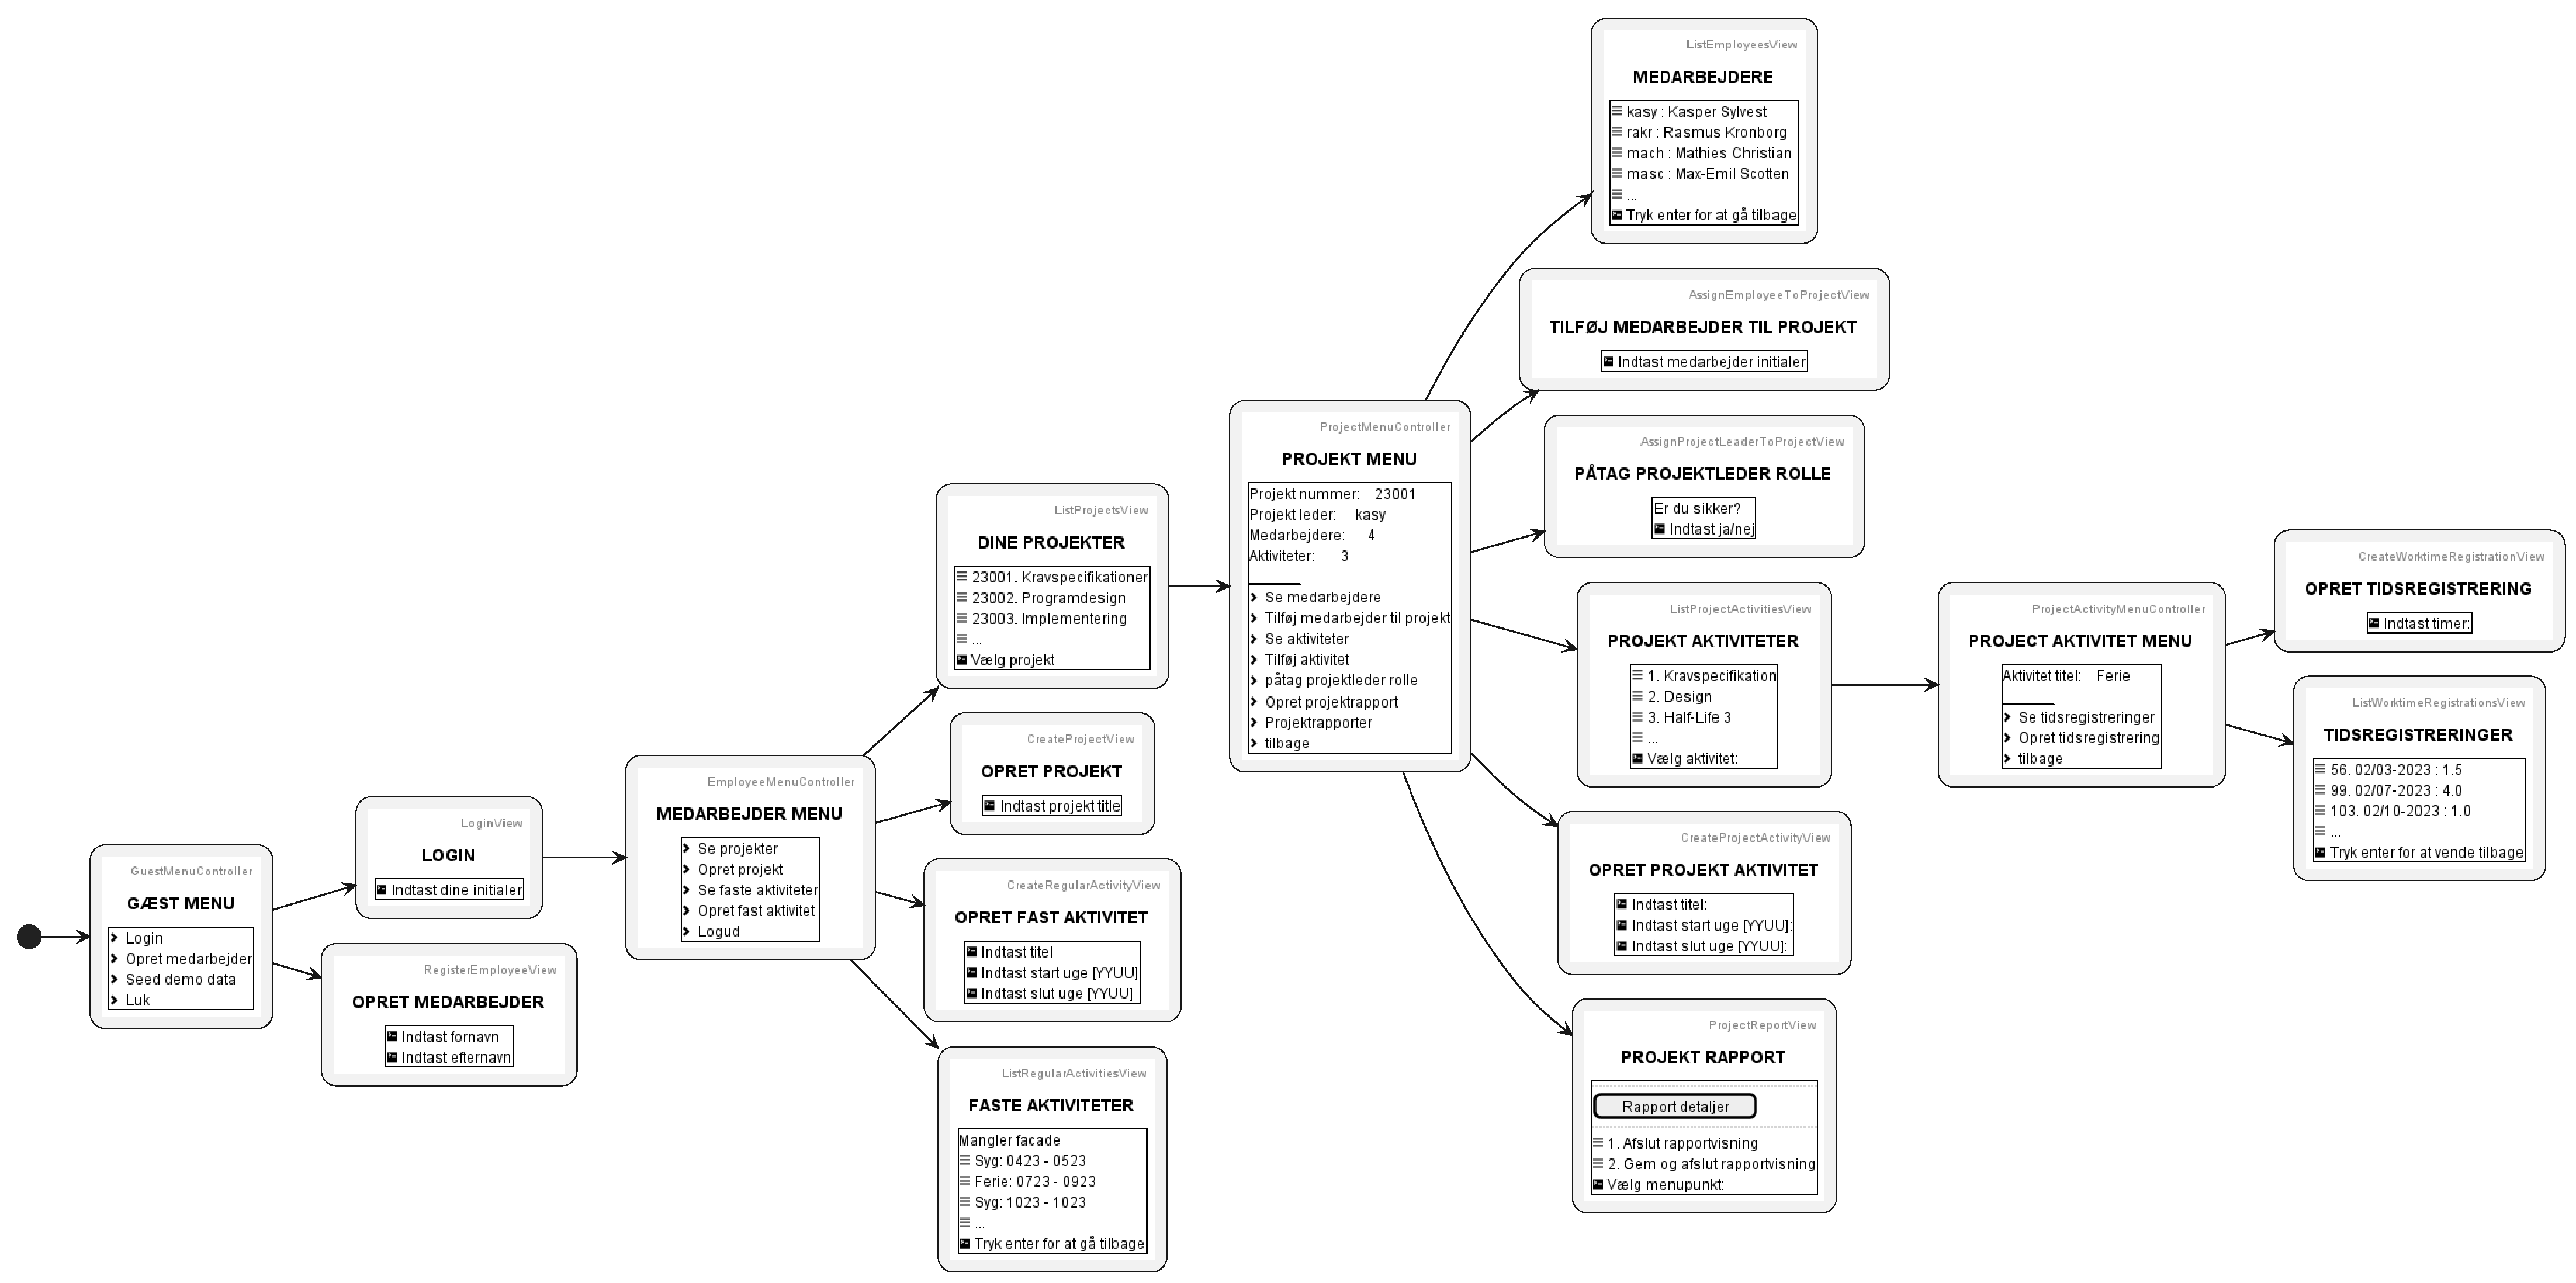
\includegraphics[width = \linewidth]{ImplementationAndTest/Diagrams/FlowCharts/flow_cli.eps}
        \label{fig:flow_cli_big}
    \end{figure}
    \section{Klassediagram over facade-laget}\label{apdx:classDiagram_facade_full}
    \begin{figure}[H]
        \centering
        \caption{Detaljeret klassediagram af facade-laget}
        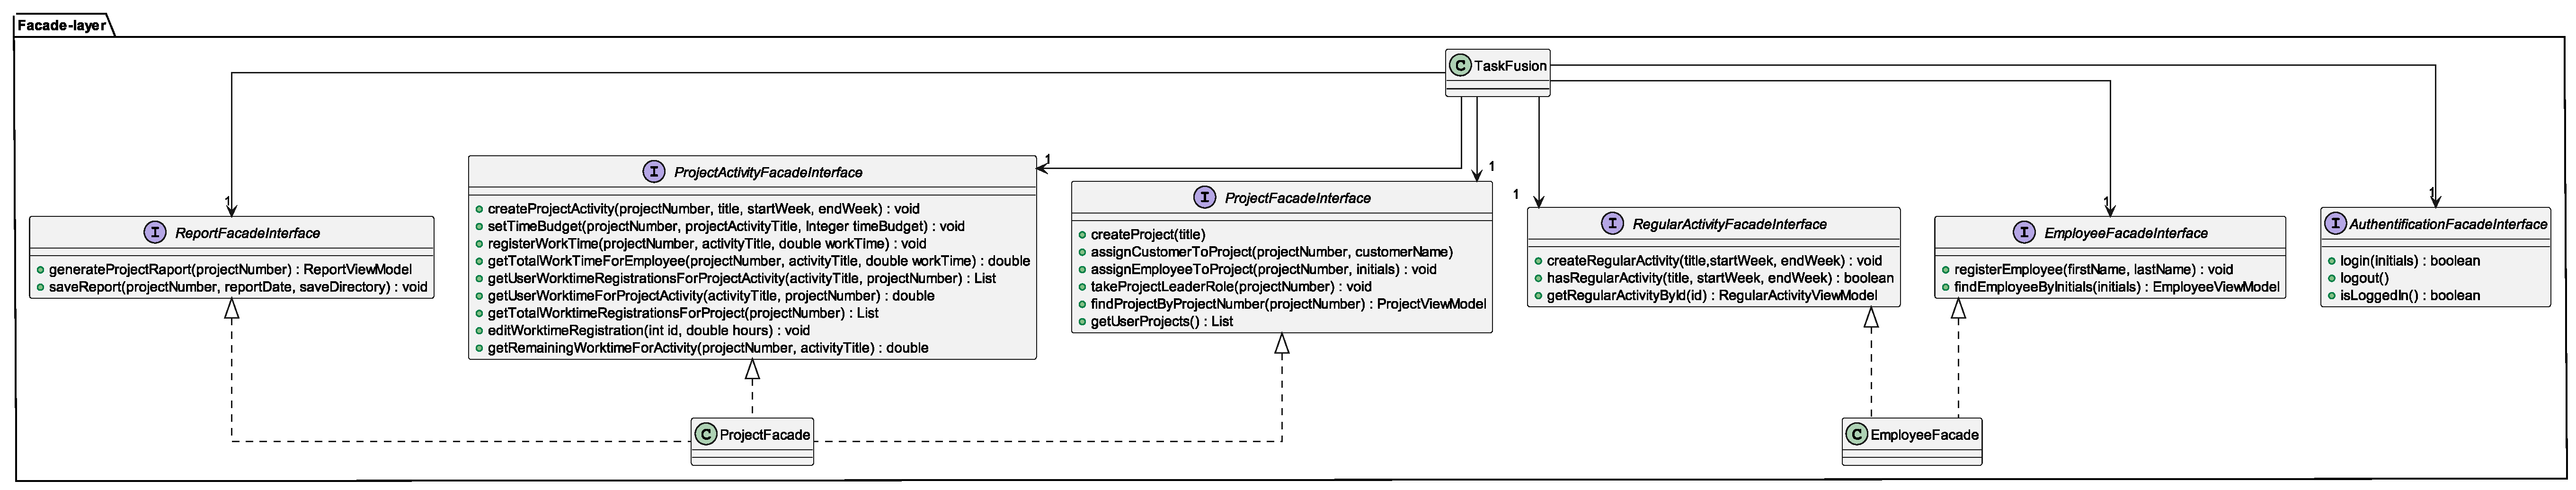
\includegraphics[width = \linewidth]{ImplementationAndTest/Diagrams/ClassDiagrams/ClassDiagram_facade_full.eps}
        \label{fig:class_facade_full}
    \end{figure}
\end{landscape}